%-----------------------------------------------------------------------------
%
%          PHYSICS  M.S.     THESIS
%          JUSTIN A. VASEL
%
%          This began as the template offered by the University of Minnesota, 
%          but I've made a few changes here and there...  
%
%          -->  snews.tex
%
%-----------------------------------------------------------------------------


\chapter{The Supernova Early Warning System}
	\label{snews_chapter}
	\vspace{-0.2in}

	\begin{quoting}
		\noindent \large ``Vision is the art of seeing things invisible." \normalsize

		--- Jonathan Swift
	\end{quoting}

	\chapterIntro{L}{ittle is known about the behavior of a star moments from death.} The mechanisms of stellar evolution are thought to be fairly well-understood thanks to a robust nuclear theory and powerfull computational models. Likewise, the after-effects of a stellar explosion are at the very least well-documented through both galactic and extra-galactic observation. But, the moments immediately preceeding and immediately following these eruptions are poorly understood because it is difficult to predict when and where a supernova will occur. 

	The idea of using the neutrino signal as an advance warning of the photon signal was fully realized with the eruption of SN 1987a, \SI{50}{\kilo\parsec} away in the Large Magellanic Cloud. A handful of neutrino detectors at the time recorded the event\cite{kii1987a,imb_1987a,baksan1987a}. A total of 26 events were observed between Kamiokande-II, IMB, and Baksan over a period of 13 seconds, all with energies $\lesssim$ \nolinebreak \eMeV{40}.

	The Supernova Early Warning System (SNEWS)\footnote{http://snews.bnl.gov} is hoping to take advantage of the neutrino signal generated during galactic core-collapse supernovae to identify the explosion before the photon signal arrives. SNEWS is a world-wide network of neutrino detectors that will listen for that distinct neutrino signal and alert the astronomical community upon its arrival. Astronomers will only have several hours to prepare their observations. 



	%% SECTION : A WORLD-WIDE NETWORK OF NEUTRINO DETECTORS
	\section{A World-Wide Network of Neutrino Detectors}
	There are at present four neutrino observatories actively participating in SNEWS: IceCube in Antarctica, Borexino and the Large Volume Detector (LVD) in Italy, and Super-Kamiokande (Super-K) in Japan. The HALO and the SNO+ experiments at SNOLAB intend to join that list soon. 
		\begin{figure}[H]
		\centering
		\includegraphics[width=1\textwidth]{snews_map}
		\caption[Map of Observatories Participating in SNEWS]{\bf Map of Observatories Participating in SNEWS. \rm At present, four observatories are actively participating (purple markers). HALO and SNO+ plan to actively participate once their triggers are in place (red markers).}
		\label{fig:snews_map}
	\end{figure}

	The experiments share a connection to a central server at Brookhaven National Laboratory. Through automated triggering software, each experiment automatically sends an alert to the central server when it believes it detected a supernova neutrino signal. If the server receives several coincident alerts, it sends the warning out to the SNEWS membership via a PGP encrypted email. 

	\begin{table}[H]
		\centering
		\caption[Summary of SNEWS Detectors]{\bf A summary of SNEWS detectors.\rm }
		\label{table:snews_detectors}
			\begin{tabular}{cccc}
				\toprule
				Detector & Type & Neutrino Sensitivity & Status \\
				\midrule
				IceCube & H$_2$O (ice) Cherenkov & $\HepParticle{\APnue}{}{}$ CC & Running \\
				Borexino & Liquid Scintillator & NC & Running \\
				LVD & Liquid Scintillator & NC & Running \\
				Super-K & H$_2$O Cherenkov 	& $\HepParticle{\APnue}{}{}$ CC & Running \\
				HALO & High-Z (Pb) & $\HepParticle{\Pnue}{}{}$ CC & In Development \\
				SNO+ & Liquid Scintillator & $\HepParticle{\APnue}{}{}$ CC & In Development \\
				\bottomrule
			\end{tabular}
	\end{table}


	%% SECTION : THE THREE P'S
	\section{The Three P's}
	In order for SNEWS to be reliable and successful, it has to adhere to ``the three P's":

	\subsection*{Prompt}
	The prompt neutrino signal may only precede the photon signal by hours or less. It is essential that SNEWS works quickly to get the word out once the neutrino signal is detected. To achieve this, the system is automated at both the detector end and the server end. Each experiment is responsible for developing its own software triggers that alert SNEWS when a supernova candidate is detected. 

	\subsection*{Pointing}
	Knowing that a supernova is about to become visible is great. What's better is knowing where to look. Detecting the directionality of incoming neutrinos is notoriously difficult. NC and CC interactions are useless because their products are nucleons or leptons whose directions are independent of that of the neutrino. Instead, elastic scattering (ES) between neutrinos and electrons ($\HepProcess{\HepParticle{\Pneutrino}{}{} + \HepParticle{\Pelectron}{}{} \to \HepParticle{\Pneutrino}{}{} + \HepParticle{\Pelectron}{}{}}$) is currently the best method because the momentum transfered to the electron points back to the direction of the incoming neutrino. Super-Kamiokande is currently the only SNEWS observatory that can provide pointing information. For a supernova at a distance of [SOME KPC] from Earth, Super-K can point with an accuracy of [NUMBER HERE] degrees[CITATION]. Triangulation between detectors around the world is technically possible, but currently the statistics associated with interactions make it too difficult. It has been proposed that the next generation of high-statistics neutrino observatories (eg. Hyper-Kamiokande) may be able to use triangulation to determine a rough location in the sky\cite{Muhlbeier2013}.

	\subsection*{Positive}
	\label{sec:snews_positive}
	\begin{wrapfigure}{r}{0.7\textwidth}
		\vspace{-0.25in}
		\centering
		\includegraphics[width=0.68\textwidth]{coincidence}
		\caption[SNEWS Rate of Accidental Alerts]{\bf SNEWS Rate of Accidental Alerts.\rm }
		\label{fig:coincidence}
		\vspace{-0.074in}
	\end{wrapfigure}
	To ensure that a SNEWS alert is taken seriously, the false-alarm rate of SNEWS must be very low. SNEWS aims for a false-alarm rate of fewer than one per century. To achieve this, SNEWS requires that each experiment has a false-alarm rate of less than once per week and that at least two detectors send an alert within ten seconds of each other. This 2-fold coincidence between detectors ensures the once-per-century threshold can be achieved, but only with three actively participating experiments. If more than three experiments are participating, the coincidence between detectors must be at least 3-fold if each detector is to maintain a once-per-week false alarm rate.



	%% SECTION : ALERTING THE ASTRONOMICAL COMMUNITY
	\section{Alerting the Astronomical Community}
	\begin{wrapfigure}{R}{0.7\textwidth}
		\centering
		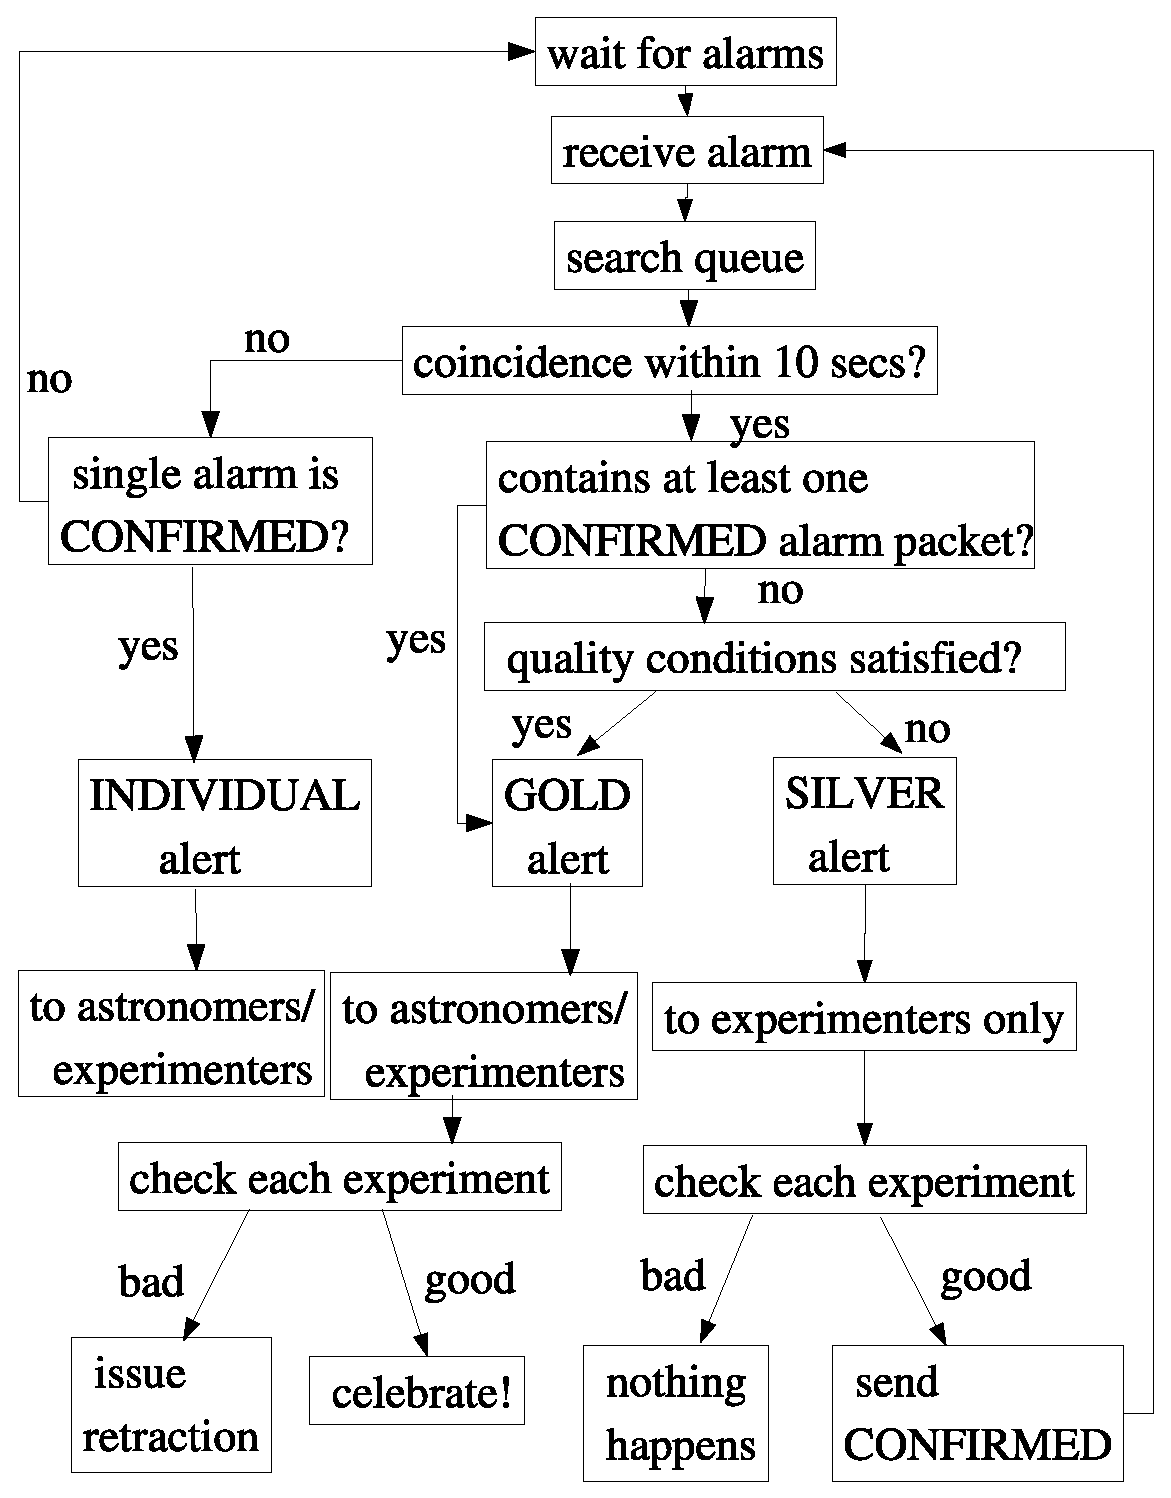
\includegraphics[width=0.68\textwidth]{snews_flowchart}
		\caption[SNEWS Flowchart]{\bf SNEWS Flowchart.\rm }
		\label{fig:flowchart}
		\vspace{0.0in}
	\end{wrapfigure}
	\filler


%-----------------------------------------------------------------------------
%-----------------------------------------------------------------------------